\documentclass{standalone}
\usepackage{tikz}
\usetikzlibrary{patterns, positioning}


\begin{document}
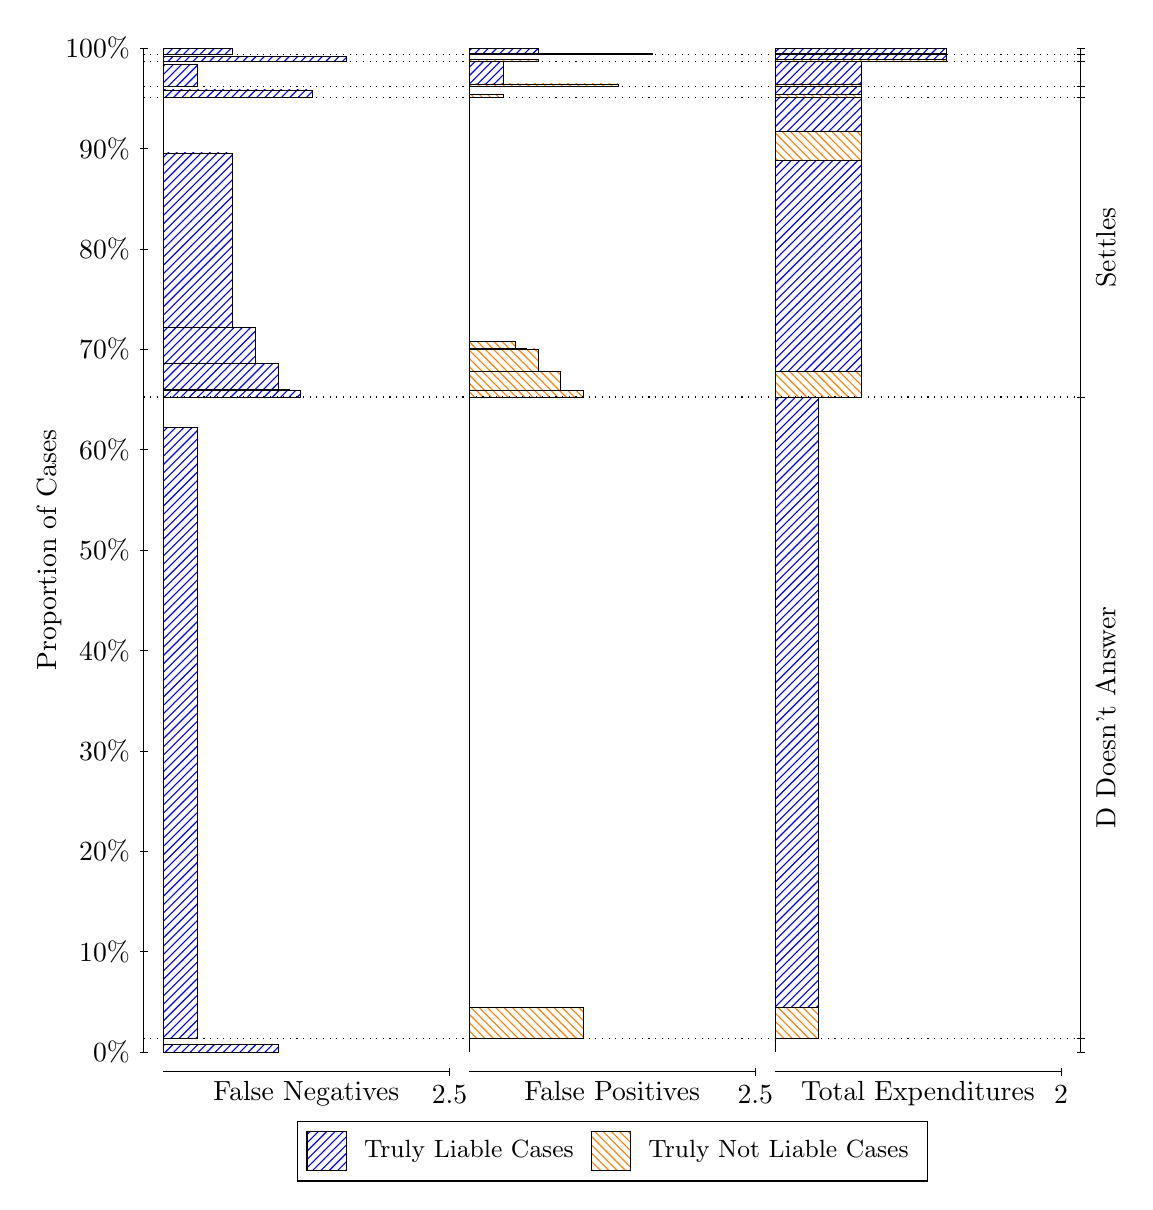
\begin{tikzpicture}
\draw[black, very thin] (1.5,1.75) -- (1.5,14.5);
\node[rotate=90, text=black, anchor=center] at (0.3, 8.125) {Proportion of Cases};
\draw[black, very thin] (1.45,1.75) -- (1.55,1.75);
\node[text=black, anchor=east] at (1.45, 1.75) {0\%};
\draw[black, very thin] (1.45,3.025) -- (1.55,3.025);
\node[text=black, anchor=east] at (1.45, 3.025) {10\%};
\draw[black, very thin] (1.45,4.3) -- (1.55,4.3);
\node[text=black, anchor=east] at (1.45, 4.3) {20\%};
\draw[black, very thin] (1.45,5.575) -- (1.55,5.575);
\node[text=black, anchor=east] at (1.45, 5.575) {30\%};
\draw[black, very thin] (1.45,6.85) -- (1.55,6.85);
\node[text=black, anchor=east] at (1.45, 6.85) {40\%};
\draw[black, very thin] (1.45,8.125) -- (1.55,8.125);
\node[text=black, anchor=east] at (1.45, 8.125) {50\%};
\draw[black, very thin] (1.45,9.4) -- (1.55,9.4);
\node[text=black, anchor=east] at (1.45, 9.4) {60\%};
\draw[black, very thin] (1.45,10.675) -- (1.55,10.675);
\node[text=black, anchor=east] at (1.45, 10.675) {70\%};
\draw[black, very thin] (1.45,11.95) -- (1.55,11.95);
\node[text=black, anchor=east] at (1.45, 11.95) {80\%};
\draw[black, very thin] (1.45,13.225) -- (1.55,13.225);
\node[text=black, anchor=east] at (1.45, 13.225) {90\%};
\draw[black, very thin] (1.45,14.5) -- (1.55,14.5);
\node[text=black, anchor=east] at (1.45, 14.5) {100\%};

\draw[black, very thin] (13.4,1.75) -- (13.4,14.5);
\draw[black, very thin] (13.35,1.75) -- (13.45,1.75);
\node[anchor=west] at (13.35, 1.75) {};
\draw[black, very thin] (13.35,1.9263) -- (13.45,1.9263);
\node[anchor=west] at (13.35, 1.9263) {};
\draw[black, very thin] (13.35,10.068) -- (13.45,10.068);
\node[anchor=west] at (13.35, 10.068) {};
\draw[black, very thin] (13.35,13.871) -- (13.45,13.871);
\node[anchor=west] at (13.35, 13.871) {};
\draw[black, very thin] (13.35,14.01) -- (13.45,14.01);
\node[anchor=west] at (13.35, 14.01) {};
\draw[black, very thin] (13.35,14.328) -- (13.45,14.328);
\node[anchor=west] at (13.35, 14.328) {};
\draw[black, very thin] (13.35,14.42) -- (13.45,14.42);
\node[anchor=west] at (13.35, 14.42) {};
\draw[black, very thin] (13.35,14.5) -- (13.45,14.5);
\node[anchor=west] at (13.35, 14.5) {};

\draw[black, very thin, pattern color=blue, pattern=north east lines] (1.75,1.75) rectangle (3.2033,1.8497);
\draw[black, very thin, pattern color=orange, pattern=north west lines] (1.75,1.8497) rectangle (1.75,1.9263);
\draw[black, very thin, pattern color=blue, pattern=north east lines] (1.75,1.9263) rectangle (2.186,9.6828);
\draw[black, very thin, pattern color=orange, pattern=north west lines] (1.75,9.6828) rectangle (1.75,10.068);
\draw[black, very thin, pattern color=blue, pattern=north east lines] (1.75,10.068) rectangle (3.494,10.155);
\draw[black, very thin, pattern color=blue, pattern=north east lines] (1.75,10.155) rectangle (3.3487,10.162);
\draw[black, very thin, pattern color=blue, pattern=north east lines] (1.75,10.162) rectangle (3.2033,10.497);
\draw[black, very thin, pattern color=blue, pattern=north east lines] (1.75,10.497) rectangle (2.9127,10.955);
\draw[black, very thin, pattern color=blue, pattern=north east lines] (1.75,10.955) rectangle (2.622,13.169);
\draw[black, very thin, pattern color=orange, pattern=north west lines] (1.75,13.169) rectangle (1.75,13.871);
\draw[black, very thin, pattern color=blue, pattern=north east lines] (1.75,13.871) rectangle (3.6393,13.967);
\draw[black, very thin, pattern color=orange, pattern=north west lines] (1.75,13.967) rectangle (1.75,14.01);
\draw[black, very thin, pattern color=blue, pattern=north east lines] (1.75,14.01) rectangle (2.186,14.293);
\draw[black, very thin, pattern color=orange, pattern=north west lines] (1.75,14.293) rectangle (1.75,14.328);
\draw[black, very thin, pattern color=blue, pattern=north east lines] (1.75,14.328) rectangle (4.0753,14.394);
\draw[black, very thin, pattern color=orange, pattern=north west lines] (1.75,14.394) rectangle (1.75,14.42);
\draw[black, very thin, pattern color=blue, pattern=north east lines] (1.75,14.42) rectangle (2.622,14.493);
\draw[black, very thin, pattern color=orange, pattern=north west lines] (1.75,14.493) rectangle (1.75,14.5);
\draw[black, very thin, pattern color=orange, pattern=north west lines] (5.6333,1.75) rectangle (5.6333,1.8266);
\draw[black, very thin, pattern color=blue, pattern=north east lines] (5.6333,1.8266) rectangle (5.6333,1.9263);
\draw[black, very thin, pattern color=orange, pattern=north west lines] (5.6333,1.9263) rectangle (7.0867,2.3114);
\draw[black, very thin, pattern color=blue, pattern=north east lines] (5.6333,2.3114) rectangle (5.6333,10.068);
\draw[black, very thin, pattern color=orange, pattern=north west lines] (5.6333,10.068) rectangle (7.0867,10.148);
\draw[black, very thin, pattern color=orange, pattern=north west lines] (5.6333,10.148) rectangle (6.796,10.396);
\draw[black, very thin, pattern color=orange, pattern=north west lines] (5.6333,10.396) rectangle (6.5053,10.679);
\draw[black, very thin, pattern color=orange, pattern=north west lines] (5.6333,10.679) rectangle (6.36,10.683);
\draw[black, very thin, pattern color=orange, pattern=north west lines] (5.6333,10.683) rectangle (6.2147,10.77);
\draw[black, very thin, pattern color=blue, pattern=north east lines] (5.6333,10.77) rectangle (5.6333,13.871);
\draw[black, very thin, pattern color=orange, pattern=north west lines] (5.6333,13.871) rectangle (6.0693,13.914);
\draw[black, very thin, pattern color=blue, pattern=north east lines] (5.6333,13.914) rectangle (5.6333,14.01);
\draw[black, very thin, pattern color=orange, pattern=north west lines] (5.6333,14.01) rectangle (7.5227,14.045);
\draw[black, very thin, pattern color=blue, pattern=north east lines] (5.6333,14.045) rectangle (6.0693,14.328);
\draw[black, very thin, pattern color=orange, pattern=north west lines] (5.6333,14.328) rectangle (6.5053,14.354);
\draw[black, very thin, pattern color=blue, pattern=north east lines] (5.6333,14.354) rectangle (5.6333,14.42);
\draw[black, very thin, pattern color=orange, pattern=north west lines] (5.6333,14.42) rectangle (7.9587,14.427);
\draw[black, very thin, pattern color=blue, pattern=north east lines] (5.6333,14.427) rectangle (6.5053,14.5);
\draw[black, very thin, pattern color=orange, pattern=north west lines] (9.5167,1.75) rectangle (9.5167,1.8266);
\draw[black, very thin, pattern color=blue, pattern=north east lines] (9.5167,1.8266) rectangle (9.5167,1.9263);
\draw[black, very thin, pattern color=orange, pattern=north west lines] (9.5167,1.9263) rectangle (10.062,2.3114);
\draw[black, very thin, pattern color=blue, pattern=north east lines] (9.5167,2.3114) rectangle (10.062,10.068);
\draw[black, very thin, pattern color=orange, pattern=north west lines] (9.5167,10.068) rectangle (10.607,10.396);
\draw[black, very thin, pattern color=blue, pattern=north east lines] (9.5167,10.396) rectangle (10.607,13.069);
\draw[black, very thin, pattern color=orange, pattern=north west lines] (9.5167,13.069) rectangle (10.607,13.442);
\draw[black, very thin, pattern color=blue, pattern=north east lines] (9.5167,13.442) rectangle (10.607,13.871);
\draw[black, very thin, pattern color=orange, pattern=north west lines] (9.5167,13.871) rectangle (10.607,13.914);
\draw[black, very thin, pattern color=blue, pattern=north east lines] (9.5167,13.914) rectangle (10.607,14.01);
\draw[black, very thin, pattern color=orange, pattern=north west lines] (9.5167,14.01) rectangle (10.607,14.045);
\draw[black, very thin, pattern color=blue, pattern=north east lines] (9.5167,14.045) rectangle (10.607,14.328);
\draw[black, very thin, pattern color=orange, pattern=north west lines] (9.5167,14.328) rectangle (11.697,14.354);
\draw[black, very thin, pattern color=blue, pattern=north east lines] (9.5167,14.354) rectangle (11.697,14.42);
\draw[black, very thin, pattern color=orange, pattern=north west lines] (9.5167,14.42) rectangle (11.697,14.427);
\draw[black, very thin, pattern color=blue, pattern=north east lines] (9.5167,14.427) rectangle (11.697,14.5);
\draw[black, dotted] (1.5,1.9263) -- (13.4,1.9263);
\draw[black, dotted] (1.5,10.068) -- (13.4,10.068);
\draw[black, dotted] (1.5,13.871) -- (13.4,13.871);
\draw[black, dotted] (1.5,14.01) -- (13.4,14.01);
\draw[black, dotted] (1.5,14.328) -- (13.4,14.328);
\draw[black, dotted] (1.5,14.42) -- (13.4,14.42);
\draw[black, very thin] (1.75,1.5) -- (5.3833,1.5);
\node[text=black, anchor=north] at (3.5667, 1.5) {False Negatives};
\draw[black, very thin] (5.3833,1.45) -- (5.3833,1.55);
\node[text=black, anchor=north] at (5.3833, 1.45) {2.5};

\draw[black, very thin] (5.6333,1.5) -- (9.2667,1.5);
\node[text=black, anchor=north] at (7.45, 1.5) {False Positives};
\draw[black, very thin] (9.2667,1.45) -- (9.2667,1.55);
\node[text=black, anchor=north] at (9.2667, 1.45) {2.5};

\draw[black, very thin] (9.5167,1.5) -- (13.15,1.5);
\node[text=black, anchor=north] at (11.333, 1.5) {Total Expenditures};
\draw[black, very thin] (13.15,1.45) -- (13.15,1.55);
\node[text=black, anchor=north] at (13.15, 1.45) {2};


\node[text=black, centered, rotate=90] at (13.72, 5.9971) {D Doesn't Answer};
\node[text=black, centered, rotate=90] at (13.72, 11.969) {Settles};





\draw (7.449999999999999,1.5) node[draw=none] (baseCoordinate) {};
\begin{scope}[align=center]
        \matrix[scale=0.5, draw=black, below=0.5cm of baseCoordinate, nodes={draw}, column sep=0.1cm]{
            \node[rectangle, draw, minimum width=0.5cm, minimum height=0.5cm, pattern color=blue, pattern=north east lines] {}; &
            \node[draw=none, font=\small, text=black] (B) {Truly Liable Cases}; &
            \node[rectangle, draw, minimum width=0.5cm, minimum height=0.5cm, pattern color=orange, pattern=north west lines] {}; &
            \node[draw=none, font=\small, text=black] (B) {Truly Not Liable Cases}; \\
            };
\end{scope}

\end{tikzpicture}
\end{document}